%
%===============>>  Ленотьева Модуль 7 <<=============
%
\setmodule{9}

%BEGIN_FOLD % ====>>_____ Занятие 1 _____<<====
\begin{class}[number=1]
	\begin{listofex}
		\item Найдите значене выражения: \( \dfrac{(a^{10})^{3}}{a^{27}} \) при \( a=6 \).
		\item Найдите значене выражения: \( \dfrac{(a^{7})^{5}}{(a^{3})^{11}} \) при \( a=11 \).
		\item Найдите значение выражения  \( \dfrac{xy+y^{2}}{8x}\cdot\dfrac{4x}{x+y} \)  при \( x = 6,5 \), \( y = -5,2 \).
		\item Найдите значение выражения  \( 10ab-(a+5b)^{2} \)  при \( a = \sqrt{10} \), \( b = \sqrt{14} \).
		\item Найдите значение выражения  \( \dfrac{8ab}{a+8b}\cdot\left( \dfrac{a}{8b}-\dfrac{8b}{a} \right) \)  при \( a = 8\sqrt{3}+7 \), \( b = \sqrt{3}-3 \).
		\item Найдите значение выражения  \( \dfrac{(a^{4})^{4}}{a^{14}} \)  при \( a = 6 \).
		\item Найдите значение выражения  \( 28ab+(2a-7b)^{2} \)  при \( a = \sqrt{15} \), \( b = \sqrt{8} \).
		\item Найдите значение выражения  \( \dfrac{a^{2}-4}{2a^{2}+4a} \)  при \( a = 0,5 \).
		\item У бабушки \( 20 \) чашек: \( 9 \) с красными цветами, остальные с синими. Бабушка наливает чай в случайно выбранную чашку. Найдите вероятность того, что это будет чашка с синими цветами.
		\item Средний рост жителя города, в котором живет Даша, равен \( 170 \) см. Рост Даши \( 173 \) см. Какое из следующих утверждений верно?
		\begin{tasks}(1)
			\task  Даша --- самая высокая девушка в городе.
			\task  Обязательно найдется девушка ниже \( 170 \) см.
			\task Обязательно найдется человек ростом менее \( 171 \) см.
			\task  Обязательно найдется человек ростом \( 167 \) см.
		\end{tasks}
		\item Средняя норма потребляемой воды в классе, в котором учится Игорь, среди мальчиков составляет \( 2,5 \) л. Игорь выпивает в день \( 2,3 \) л воды. Какое из следующих утверждений верно?
		\begin{tasks}(1)
			\task  Обязательно найдется мальчик, который выпивает \( 2,6 \) л в день.
			\task Все мальчики, кроме Игоря, выпивают в день по \( 2,5 \) л воды.
			\task  Обязательно найдется мальчик в классе, который пьет больше, чем \( 2,5 \) л в день.
			\task Обязательно найдется мальчик в классе, который выпивает ровно \( 2,5 \) л в день.
		\end{tasks}
	\newpage
		\item На рисунках изображены графики функций вида \( y=kx + b \). Установите соответствие между знаками коэффициентов \( k \) и \( b \) и графиками функций.
		% TODO: \usepackage{graphicx} required
		
		
		\begin{figure}[h]
			\center{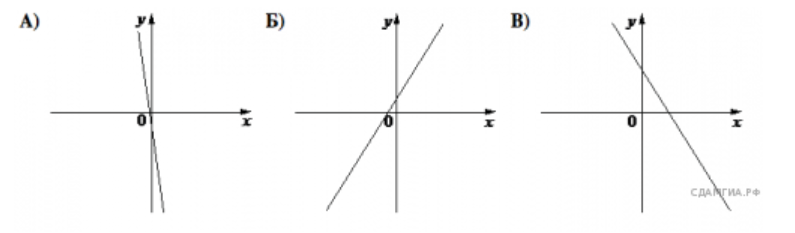
\includegraphics[align=t, width=\linewidth]{../../../../../exercises/lists/pics/leontevaM9L3-1}}
		\end{figure}
		\begin{tasks}(3)
			\task \( k<0 \), \( b<0 \)
			\task \( k<0 \), \( b>0 \)
			\task \( k>0 \), \( b>0 \)
		\end{tasks}
		\item Найдите значение \( k \) по графику функции \( y= \dfrac{k}{x} \),  изображенному на рисунке.
	\begin{figure}[h]
		\center{
				% TODO: \usepackage{graphicx} required
		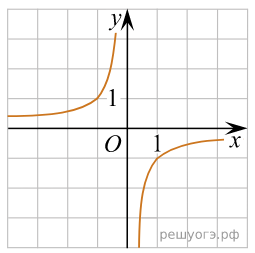
\includegraphics[align=t, width=0.3\linewidth]{../../../../../exercises/lists/pics/leontevaM9L3-2}
		}
	\end{figure}
		\newpage
		\item Установите соответствие между функциями и их графиками.
		\begin{tasks}(3)
			\task \( y=-3x \)
			\task \( y=-\dfrac{1}{3}x \)
			\task \( y=\dfrac{1}{3}x \)
		\end{tasks}
	\begin{figure}[h]
		\center{
			% TODO: \usepackage{graphicx} required
	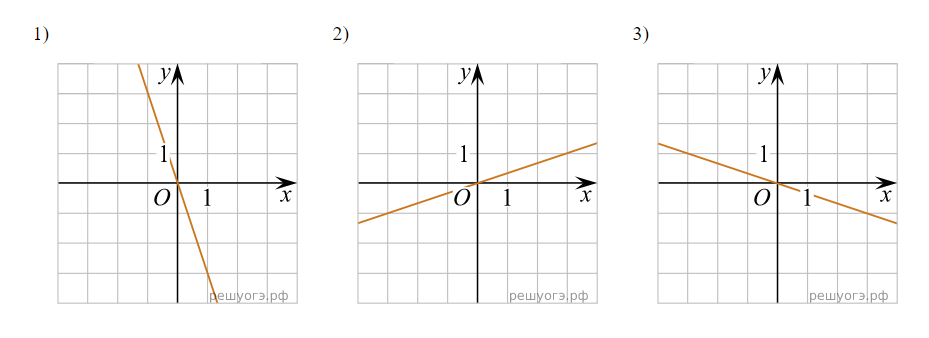
\includegraphics[align=t, width=\linewidth]{../../../../../exercises/lists/pics/leontevaM9L3-3}
	}
	\end{figure}
	\item Зная длину своего шага, человек может приближённо подсчитать пройденное им расстояние \( s \) по формуле \( s  =  nl \), где \( n \)  — число шагов, \( l \)  — длина шага. Какое расстояние прошёл человек, если \( l  =  50 \) см, \( n  =  1100 \)? Ответ выразите в километрах.
	\item Укажите решение неравенства \( (x+4)(x-8)>0 \)
	\begin{figure}[h]
		\center{
			% TODO: \usepackage{graphicx} required
	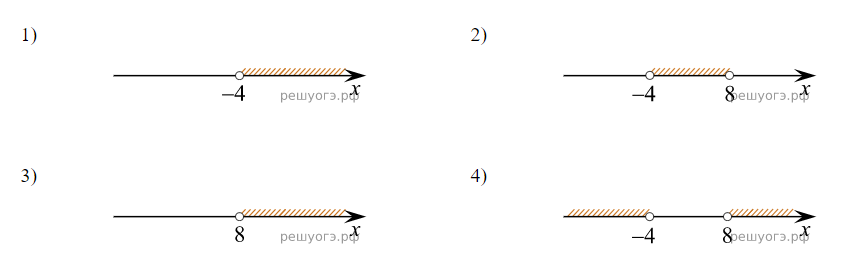
\includegraphics[align=t, width=\linewidth]{../../../../../exercises/lists/pics/leontevaM9L3-4}
	}
	\end{figure}
	\item Катеты прямоугольного треугольника равны \( \sqrt{15}  \) и \( 1 \). Найдите синус наименьшего угла этого треугольника.
	\item На окружности с центром \( O \) отмечены точки \( A \) и \( B \) так, что \( \angle AOB = 8\degree \). Длина меньшей дуги \( AB \) равна \( 99 \). Найдите длину большей дуги.
	\item Периметр квадрата равен \( 56 \). Найдите площадь квадрата.
	\item Какие из данных утверждений верны? Запишите их номера.
	\begin{tasks}(1)
		\task  У равнобедренного треугольника есть ось симметрии.
		\task  Если в параллелограмме диагонали равны и перпендикулярны, то этот параллелограмм --- квадрат.
		\task   Две окружности пересекаются, если радиус одной окружности больше радиуса другой окружности.
	\end{tasks}
	\end{listofex}
\end{class}
%END_FOLD

%BEGIN_FOLD % ====>>_____ Занятие 2 _____<<====
\begin{class}[number=2]
	\begin{listofex}
		\item Найдите значение выражения \( \dfrac{a^{2}-4b^{2}}{2ab}:\left( \dfrac{1}{2b}-\dfrac{1}{a} \right)  \) при \(a= \mfrac{2}{15}{19} \),\\\ \( b=\mfrac{5}{2}{19} \).
		\item Найдите значение выражения \( 2b+\dfrac{^{2}}{b} \) при \( a=90 \), \( b=48 \).
		\item Найдите значение выражения \( \dfrac{(a^{3})^{4}}{a^{9}} \) при \( a=3 \)
		\item Упростите выражение \( (2-c)^{2}-c(c+4) \), найдите его значение при \( c=0,5 \). В ответ запишите полученное число.
		\item Какое из данных ниже чисел является значением выражения \\\ \( \sqrt{6\cdot40}\cdot\sqrt{90} \) \begin{tasks}(4)
			\task \( 60\sqrt{6} \)
			\task \( 60\sqrt{30} \)
			\task \( 180\sqrt{2} \)
			\task \( 120\sqrt{3} \)
		\end{tasks}
		\item Определите вероятность того, что при бросании игрального кубика (правильной кости) выпадет менее \( 4 \) очков.
		\item Стрелок 4 раза стреляет по мишеням. Вероятность попадания в мишень при одном выстреле равна \( 0,6 \). Найдите вероятность того, что стрелок первые \( 3 \) раза попал в мишени, а последний раз промахнулся.
		\item Игральную кость бросают дважды. Найдите вероятность того, что хотя бы раз выпало число, большее \( 3 \).
		\item 
			График какой из приведенных ниже функций изображен на рисунке?
		\begin{figure}[h]
			\center{
				% TODO: \usepackage{graphicx} required
		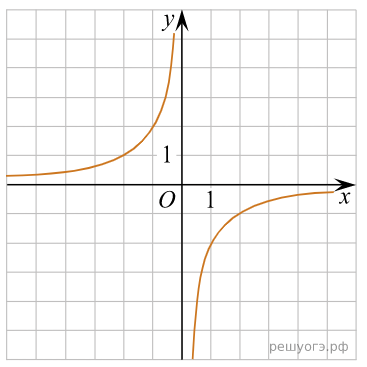
\includegraphics[align=t, width=0.3\linewidth]{../../../../../exercises/lists/pics/leontevaM9L4-1}}
		\end{figure}
		
	\begin{tasks}(4)
		\task \( y=-\dfrac{2}{x} \)
		\task \( y=\dfrac{2}{x} \)
		\task \( y=-\dfrac{1}{2x} \)
		\task \( y=\dfrac{1}{2x} \)
	\end{tasks}
	\item На рисунке изображён график квадратичной функции \( y  =  f(x)  \).Какие из следующих утверждений о данной функции неверны? Запишите их номера.
	\begin{figure}[h]
		\center{
			% TODO: \usepackage{graphicx} required
	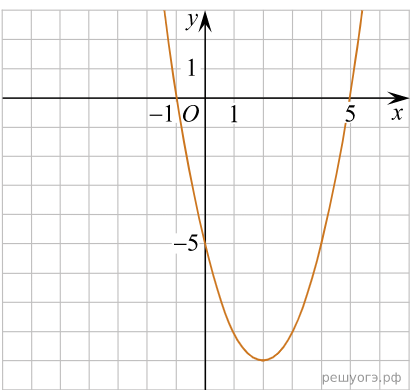
\includegraphics[align=t, width=0.3\linewidth]{../../../../../exercises/lists/pics/leontevaM9L4-2}}
	\end{figure}
	
	\begin{tasks}(1)
		\task \( f(x)< 0  \) при \( -1<x<5 \).
		\task  Функция возрастает на промежутке \( [2;+\infty] \)
		\task Наименьшее значение функции равно \( -5 \).
	\end{tasks}
	\item У Тани есть теннисный мячик. Она со всей силы бросила его об асфальт. После первого отскока мячик подлетел на высоту \( 360 \) см, а после каждого следующего отскока от асфальта подлетал на высоту в три раза меньше предыдущей. После какого по счёту отскока высота, на которую подлетит мячик, станет меньше \( 15 \) см?
	\item 
	\begin{minipage}[t]{\bodywidth}
		В кафе есть только квадратные столики, за каждый из которых могут сесть \( 4 \) человека. Если сдвинуть два квадратных столика, то получится стол, за который могут сесть \( 6 \) человек. На рисунке изображён случай, когда сдвинули \( 3 \) квадратных столика вдоль одной линии. В этом случае получился стол, за который могут сесть \( 8 \) человек. Сколько человек может сесть за стол, который получится, если сдвинуть \( 16 \) квадратных столиков вдоль одной линии?
	\end{minipage}
	\hspace{0.02\linewidth}
	\begin{minipage}[t]{\picwidth}
		% TODO: \usepackage{graphicx} required
		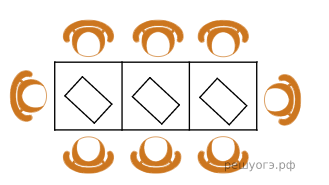
\includegraphics[align=t, width=\linewidth]{../../../../../exercises/lists/pics/leontevaM9L4-4}
	\end{minipage}
	\item В амфитеатре \( 14 \) рядов, причём в каждом следующем ряду на одно и то же число мест больше, чем в предыдущем. В пятом ряду \( 27 \) мест, а в восьмом ряду \( 36 \) мест. Сколько мест в последнем ряду амфитеатра?
	\item Найдите угол \( АВС \) равнобедренной трапеции \( ABCD \), если диагональ \( АС \) образует с основанием \( AD \) и боковой стороной \( CD \) углы, равные \( 20\degree \) и \( 100\degree \) соответственно.
	\item В треугольнике \( ABC  \) угол \( C = 90\degree \), \( BC=12 \), \( \sin A=\dfrac{ 4,}{11} \).  Найдите \( AB \).
	\item Касательные в точках \( A \) и \( B \) к окружности с центром \( O \) пересекаются под углом \( 88\degree \). Найдите угол \( ABO \). Ответ дайте в градусах.
	\end{listofex}
\end{class}
%END_FOLD

%BEGIN_FOLD % ====>>_ Домашняя работа 1 _<<====
\begin{homework}[number=1]
	\begin{listofex}
		\item[] Маша купила большой лист формата А0 для своего проекта. Однако, для выполнения проекта Маше нужны листы формата \( A1 \), \( A2 \), \( A3 \), \( A4 \) и т.д. Маша поняла, что необязательно покупать эти листы отдельно в магазине, ведь, если разрезать лист формата \( A0  \) пополам, то получится лист формата \( A1 \), а если разрезать лист формата \( A1 \) пополам, то получится лист формата \( A2 \) и т.д. Маша также заметила, что каждый лист имеет форму прямоугольника и у всех листов, которые она получила, то есть листов \( A0 \), \( A1 \), \( A2 \) и т.д. совершенно одинаковое отношение длины к ширине. 
		Так, при уменьшении размера листа расположение текста и его форма сохраняются, а вот размер шрифта меняется.
		\begin{figure}[h]
			\center{
				% TODO: \usepackage{graphicx} required
		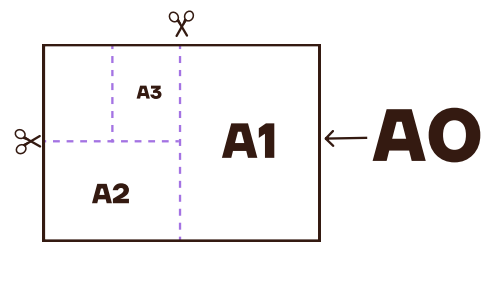
\includegraphics[align=t, width=0.5\linewidth]{../../../../../exercises/lists/pics/leontevaM9H2-4}}
		\end{figure}
		\item[] В таблице ниже Маша выписала длину и ширину различных листов бумаги (в миллиметрах),
		начиная от \( A3 \), заканчивая \( A0 \).
		\begin{figure}[h]
			\center{
				% TODO: \usepackage{graphicx} required
		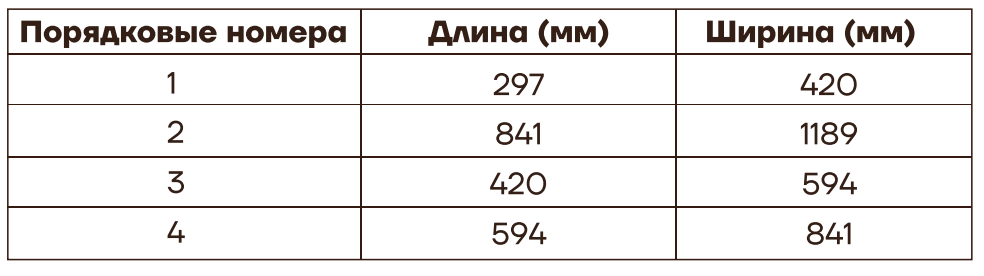
\includegraphics[align=t, width=0.5\linewidth]{../../../../../exercises/lists/pics/leontevaM9H2-5}
		}
		\end{figure}
		\item В таблице ниже представлены различные форматы листов. Установите соответствие между форматами листов и их размерами. В ответ запишите последовательность цифр без пробелов и запятых.
		\begin{figure}[h]
			\center{
				% TODO: \usepackage{graphicx} required
		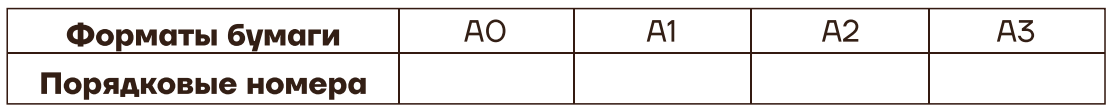
\includegraphics[align=t, width=0.5\linewidth]{../../../../../exercises/lists/pics/leontevaM9H2-6}
		}
		\end{figure}
		\item Маша разрезала лист формата \( A0 \) пополам, а затем получившиеся половинки также разрезала пополам до тех пор, пока не получила очень много листов формата \( A6 \). Определите количество листов формата \( A6 \), которые получила Маша.
		\item Вычислите длину меньшей стороны листа формата \( A4 \).
		\item Найдите площадь листа \( A1 \). Ответ дайте в см\( ^{2} \).
		\item Бумагу формата \( A3 \) упаковали в пачки по \( 500 \) листов. Найдите массу пачки, если
		масса бумаги площади \( 1 \) кв. м равна \( 80 \) г? Ответ дайте в граммах.
		\item Найдите значение выражения \( 7,8 + 8,9 \).
		\item На координатной прямой отмечено число \( a \). Какое из утверждений для этого числа
		является верным?
		\begin{figure}[h]
			\center{
				% TODO: \usepackage{graphicx} required
		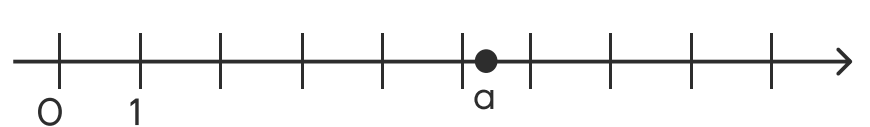
\includegraphics[align=t, width=0.3\linewidth]{../../../../../exercises/lists/pics/leontevaM9H2-7}
		}
		\end{figure}
		\begin{tasks}(4)
			\task \( 4 - a > 0 \)
			\task \( a-7 < 0 \)
			\task \( a-8 > 0 \)
			\task \( 8 - a > 0 \)
		\end{tasks}
		\item Найдите значение выражения \( \dfrac{a^{5}\cdot a^{17}}{a^{19}} \) при \( a=2 \).
		\item Решите уравнение \( \dfrac{x+3}{x+4}=3 \)
		\item В среднем из \( 100 \) карманных фонариков, поступивших в продажу, четыре
		неисправных. Найдите вероятность того, что выбранный наудачу в магазине
		фонарик окажется исправен.
		\item Изображены графики функций \( y = ax^{2} + bx + c \). Сопоставьте графики со знаками
		коэффициентов \( a \) и \( c \).
		\begin{figure}[h]
			\center{
				% TODO: \usepackage{graphicx} required
		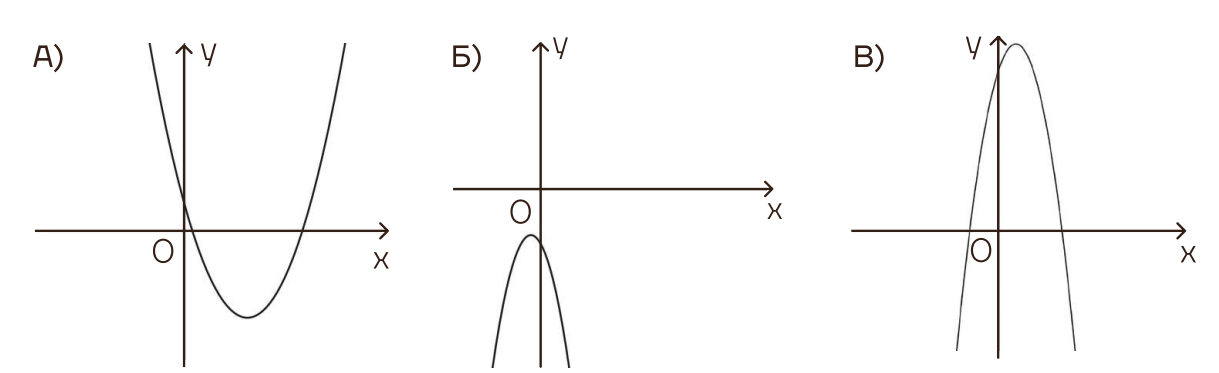
\includegraphics[align=t, width=\linewidth]{../../../../../exercises/lists/pics/leontevaM9H2-8}
		}
		\end{figure}
		\begin{tasks}(3)
			\task \( a<0 \), \( c>0 \)
			\task \( a>0 \), \( c>0 \)
			\task \( a<0 \), \( c<0 \)
		\end{tasks}
		\item Мощность постоянного тока (в ваттах) вычисляется по формуле \( P = I^{2}R \) , где \( I \) – сила тока (в амперах), \( R \) – сопротивление (в омах). Пользуясь этой формулой, найдите сопротивление \( R \), если мощность составляет \( 15,75 \) Вт, а сила тока равна \( 1,5 \) \( A \). Ответ дайте в омах.
		\item Укажите решение неравенства \( (x-7)(x+1)\leq0 \).
		\begin{tasks}(2)
			\task \( [-1;+\infty) \)
			\task \( [-1;7] \)
			\task \( (-\infty;-1] \) \( \bigcup \) \( [7;+\infty) \)
			\task \( [7;+\infty) \)
		\end{tasks}
		\item В амфитеатре \( 14 \) рядов. В первом ряду \( 16 \) мест, а в каждом следующем на \( 2  \) места
		больше, чем в предыдущем. Сколько всего мест в амфитеатре?
		\item Сторона треугольника равна \( 16 \), а высота, проведённая к этой стороне, равна A.
		Найдите площадь этого треугольника.
		\item 
		\begin{minipage}[t]{\bodywidth}
			Центр окружности, описанной около треугольника \( ABC \), лежит на стороне \( AB \). Радиус окружности равен \( 14,5 \). Найдите \( AC \), если \( BC = 21 \).
		\end{minipage}
		\hspace{0.02\linewidth}
		\begin{minipage}[t]{\picwidth}
			% TODO: \usepackage{graphicx} required
			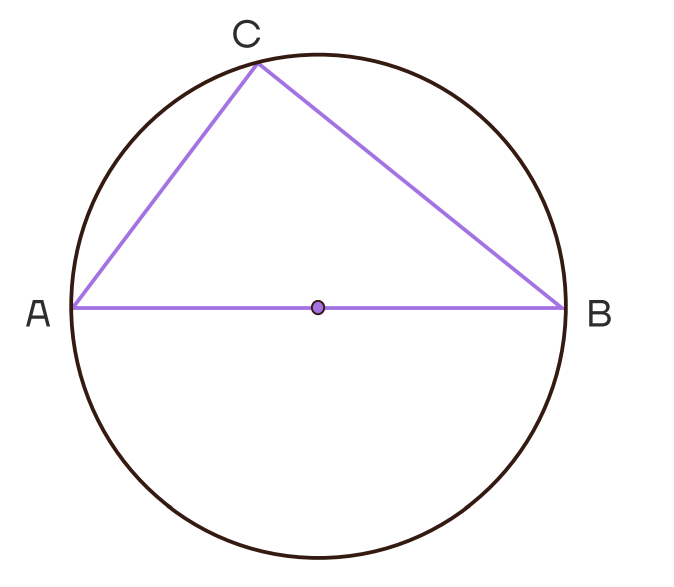
\includegraphics[align=t, width=\linewidth]{../../../../../exercises/lists/pics/leontevaM9H2-10}
		\end{minipage}
		\item 
		\begin{minipage}[t]{\bodywidth}
			В равнобедренной трапеции известна высота, меньшее основание и угол при
		основании (см. рисунок). Найдите большее основание.
		\end{minipage}
		\hspace{0.02\linewidth}
		\begin{minipage}[t]{\picwidth}
			% TODO: \usepackage{graphicx} required
			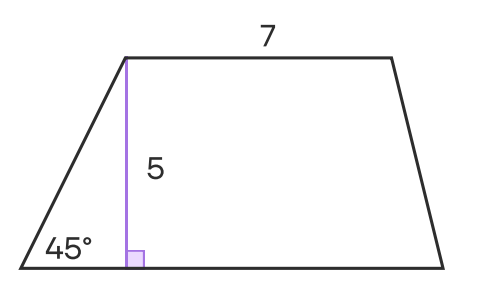
\includegraphics[align=t, width=\linewidth]{../../../../../exercises/lists/pics/leontevaM9H2-9}
		\end{minipage}
		\item 
		\begin{minipage}[t]{\bodywidth}
			 На клетчатой бумаге с размером клетки \(  1\times 1 \) изображена трапеция. Найдите
		длину её средней линии.
		\end{minipage}
		\hspace{0.02\linewidth}
		\begin{minipage}[t]{\picwidth}
			% TODO: \usepackage{graphicx} required
			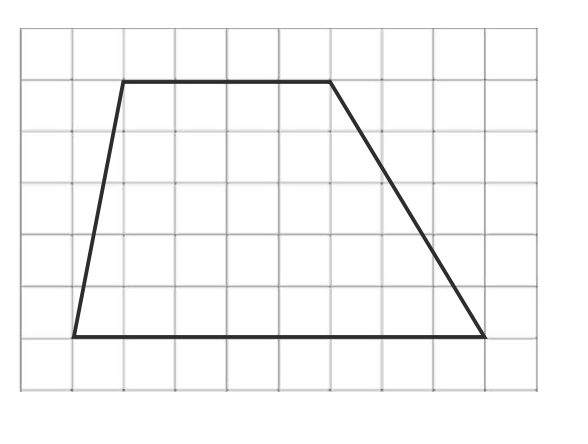
\includegraphics[align=t, width=\linewidth]{../../../../../exercises/lists/pics/leontevaM9H2-11}
		\end{minipage}
		\item Какие из следующих утверждений верны? \begin{tasks}(1)
			\task В треугольнике против меньшего угла лежит большая сторона.
			
			\task Если один угол треугольника больше \( 120\degree \), то два других его угла меньше \( 30\degree \).
			
			\task Если все стороны треугольника меньше \( 1 \), то и все его высоты меньше \(  1 \).
			
			\task Сумма острых углов прямоугольного треугольника не превосходит \( 90\degree \).
		\end{tasks}
	\end{listofex}
\end{homework}
%END_FOLD

%BEGIN_FOLD % ====>>_____ Занятие 3 _____<<====
\begin{class}[number=3]
	\begin{listofex}
		\item Уравнение \( x ^{2}+ px + q=0 \) имеет корни \( -5; 7 \). Найдите \( q \). 
		\item Найдите корень уравнения \( -1 - 3x = 2x + 1 \).
		\item При проведении опыта вещество равномерно охлаждали в течение \( 10 \) минут. При этом каждую минуту температура вещества уменьшалась на \( 6 \) \( \degree C \). Найдите температуру вещества (в градусах Цельсия) через \( 4 \) минуты после начала проведения опыта, если его начальная температура составляла \( -7\) \( \degree C  \).
		\item 
		\begin{minipage}[t]{\bodywidth}
			На прямой \( AB \) взята точка \( M \). Луч \( MD \) --- биссектриса угла \( CMB \). Известно, что \( \angle DMC =  60\degree \)  . Найдите угол \( CMA \). Ответ дайте в градусах.
		\end{minipage}
		\hspace{0.02\linewidth}
		\begin{minipage}[t]{\picwidth}
			% TODO: \usepackage{graphicx} required
			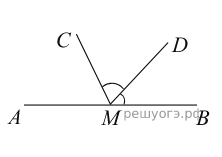
\includegraphics[align=t, width=\linewidth]{../../../../../exercises/lists/pics/leontevaM9H2-1}
		\end{minipage}
		\item 
		\begin{minipage}[t]{\bodywidth}
			Радиус окружности с центром в точке \( O \) равен \( 40 \), длина хорды \( AB \) равна \( 64 \) (см. рис.). Найдите расстояние от хорды \( AB \) до параллельной ей касательной \( k \).
		\end{minipage}
		\hspace{0.02\linewidth}
		\begin{minipage}[t]{\picwidth}
			% TODO: \usepackage{graphicx} required
			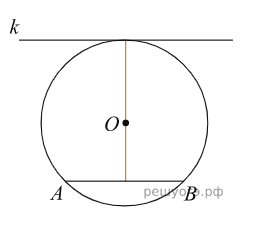
\includegraphics[align=t, width=\linewidth]{../../../../../exercises/lists/pics/leontevaM9H2-2}
		\end{minipage}
		\item Два катета прямоугольного треугольника равны \( 4 \) и \( 9 \). Найдите площадь этого треугольника.
		\item 
		\begin{minipage}[t]{\bodywidth}
			Найдите площадь треугольника, изображённого на рисунке.
		\end{minipage}
		\hspace{0.02\linewidth}
		\begin{minipage}[t]{\picwidth}
			% TODO: \usepackage{graphicx} required
			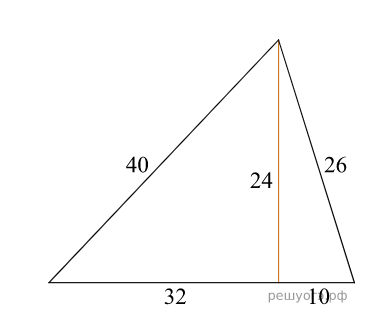
\includegraphics[align=t, width=\linewidth]{../../../../../exercises/lists/pics/leontevaM9H2-3}
		\end{minipage}
		\item Укажите номера верных утверждений.
		\begin{tasks}(1)
			\task  Медиана равнобедренного треугольника, проведённая из вершины угла, противолежащего основанию, делит этот угол пополам.
			\task Не существует прямоугольника, диагонали которого взаимно перпендикулярны.
			\task В плоскости для точки, лежащей вне круга, расстояние до центра круга больше его радиуса.
		\end{tasks}
		
	\end{listofex}
\end{class}
%END_FOLD

%BEGIN_FOLD % ====>>_____ Занятие 4 _____<<====
\begin{class}[number=4]
	\begin{listofex}
		\item  Занятие 4
	\end{listofex}
\end{class}
%END_FOLD

%BEGIN_FOLD % ====>>_ Домашняя работа 2 _<<====
\begin{homework}[number=2]
	\begin{listofex}
		\item Домашняя работа 2
	\end{listofex}
\end{homework}
%END_FOLD

%BEGIN_FOLD % ====>>_____ Занятие 5 _____<<====
\begin{class}[number=5]
	\begin{listofex}
		\item Занятие 5
	\end{listofex}
\end{class}
%END_FOLD

%BEGIN_FOLD % ====>>_____ Занятие 6 _____<<====
\begin{class}[number=6]
	\begin{listofex}
		\item Найдите значение выражения \( \dfrac{(a^{3})^{4}}{a^{9}} \) при \( a=3 \)
		\item Сократите дробь \( \left( \dfrac{a+b}{a^{2}-ab}-\dfrac{1}{a} \right):\dfrac{b}{b-a} \) при \( a=0,5 \),\( b=\sqrt{7}-2 \).
		\item Определите вероятность того, что при бросании игрального кубика (правильной кости) выпадет менее \( 4 \) очков.
		\item Игральную кость бросают дважды. Найдите вероятность того, что хотя бы раз выпало число, большее \( 3 \).
		
		
		\item В фирме такси в данный момент свободно \( 10 \) машин: \( 5 \) чёрных, \(  1 \) жёлтая
		и \( 4 \) зелёных. По вызову выехала одна из машин, случайно оказавшаяся
		ближе всего к заказчику. Найдите вероятность того, что к нему приедет жёлтое такси.
		
		
		\item В лыжных гонках участвуют 11 спортсменов из России, 6 спортсменов
		из Норвегии и 3 спортсмена из Швеции. Порядок, в котором спортсмены стартуют, определяется жребием. Найдите вероятность того, что первым будет стартовать спортсмен из России.
		
		\newpage
		\item 
		График какой из приведенных ниже функций изображен на рисунке?
		\\\
		\begin{figure}[!h]
			\center{
				% TODO: \usepackage{graphicx} required
		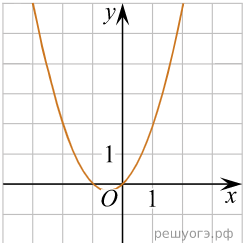
\includegraphics[align=t, width=0.25\linewidth]{../../../../../exercises/lists/pics/leontevaM9L5-1}
		}
		\end{figure}
		
		\begin{tasks}(4)
			\task \( y=x^{2}- x \)
			\task \( y=-x^{2}- x \)
			\task \( y=x^{2}+ x \)
			\task \( y=-x^{2}+ x \)
		\end{tasks}
		\item 
		График какой из приведенных ниже функций изображен на рисунке?
		\\\
		
		\begin{figure}[!h]
			\center{
				% TODO: \usepackage{graphicx} required
				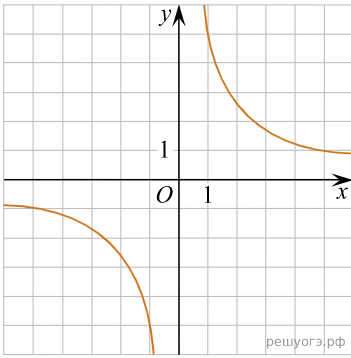
\includegraphics[align=t, width=0.25\linewidth]{../../../../../exercises/lists/pics/leontevaM9L5-2}
				
		}
		\end{figure}
		
		\begin{tasks}(4)
			\task \( y=-\dfrac{5}{x} \)
			\task \( y=-\dfrac{1}{5x} \)
			\task \( y=\dfrac{5}{x} \)
			\task \( y=\dfrac{1}{5x} \)
		\end{tasks}
		\item Найдите угол \( ABC \) равнобедренной трапеции \( ABCD \), если диагональ \( AC \) образует с основанием \( AD \) и боковой стороной \( CD \) углы, равные \( 20\degree \) и \( 100\degree \) соответственно.
		
		\item 
		\begin{minipage}[t]{\bodywidth}
			Прямые \( m \) и \( n \) параллельны. Найдите \( \angle 3 \), если \( \angle 1 = 42\degree \), \( \angle 2 = 73\degree \). Ответ дайте в градусах.
		\end{minipage}
		\hspace{0.02\linewidth}
		\begin{minipage}[t]{\picwidth}
			% TODO: \usepackage{graphicx} required
			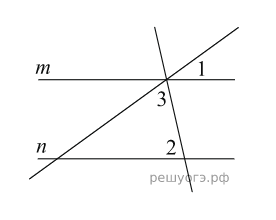
\includegraphics[align=t, width=\linewidth]{../../../../../exercises/lists/pics/leontevaM9L5-3}
		\end{minipage}
		
	\end{listofex}
\end{class}
%END_FOLD

%BEGIN_FOLD % ====>>_ Домашняя работа 3 _<<====
\begin{homework}[number=3]
	\begin{listofex}
		\item Найдите значение выражения \( a(a+1)-(a-3)^{2} \) при \( a=-1 \).
		\item Найдите значение выражения \( 28ab+(2a-7b)^{2} \) при \( a=\sqrt{15} \), \( b=\sqrt{8} \).
		\item Найдите значение выражения \( \left( a+\dfrac{1}{a}+2 \right)\cdot\dfrac{1}{a+1} \) при \( a=2 \).
		\item Найдите значение выражения \( \dfrac{5ab}{5ab-8a^{2}} \) при \( a=3 \), \( b=8 \).
		\item Найдите значение выражения \( 6a+\dfrac{2c-6a^{2}}{a} \) при \( a=12 \), \( c=15 \).
		\item Найдите значение выражения \( \dfrac{a+x}{a}:\dfrac{ax+x^{2}}{a^{2}} \) при \( a=56 \), \( b=40 \).
		\item 
		\begin{minipage}[t]{\bodywidth}
			Найдите тангенс угла \( AOB \), изображённого на рисунке.
		\end{minipage}
		\hspace{0.02\linewidth}
		\begin{minipage}[t]{\picwidth}
			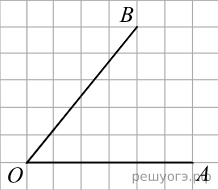
\includegraphics[align=t, width=\linewidth]{../../../../../exercises/lists/pics/leontevaM9H3-4}
		\end{minipage}
		\item 
		\begin{minipage}[t]{\bodywidth}
			В параллелограмме \( ABCD \) диагональ \( AC \) в \( 2 \) раза больше стороны \( AB \) и \( \angle ACD=111 \degree \). Найдите угол между диагоналями параллелограмма. Ответ дайте в градусах.
		\end{minipage}
		\hspace{0.02\linewidth}
		\begin{minipage}[t]{\picwidth}
			% TODO: \usepackage{graphicx} required
			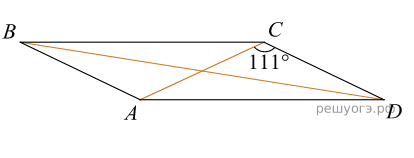
\includegraphics[align=t, width=\linewidth]{../../../../../exercises/lists/pics/leontevaM9H3-1}
		\end{minipage}
	 	\item 
	 	\begin{minipage}[t]{\bodywidth}
	 		Найдите больший угол равнобедренной трапеции \( ABCD \), если диагональ \( AC \) образует с основанием \( AD \) и боковой стороной \( AB \) углы, равные \( 62\degree \) и \( 9\degree \) соответственно. Ответ дайте в градусах.
	 	\end{minipage}
	 	\hspace{0.02\linewidth}
	 	\begin{minipage}[t]{\picwidth}
			% TODO: \usepackage{graphicx} required
			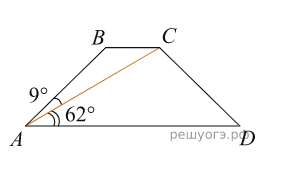
\includegraphics[align=t, width=\linewidth]{../../../../../exercises/lists/pics/leontevaM9H3-2}
	 	\end{minipage}
 		
		\item В трапецию, сумма длин боковых сторон которой равна \( 24 \), вписана окружность. Найдите длину средней линии трапеции.
		\item 
		\begin{minipage}[t]{\bodywidth}
			Прямая касается окружности в точке \( K \). Точка \( O \)  --- центр окружности. Хорда \( KM \) образует с касательной угол, равный \( 32\degree \). Найдите величину угла \( OMK \). Ответ дайте в градусах.
		\end{minipage}
		\hspace{0.02\linewidth}
		\begin{minipage}[t]{\picwidth}
				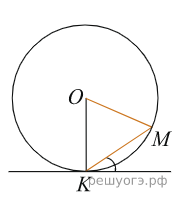
\includegraphics[align=t, width=\linewidth]{../../../../../exercises/lists/pics/leontevaM9H3-3}
		\end{minipage}
		\item Найдите площадь кругового сектора, если радиус круга равен \( 3 \), а угол сектора равен \( 120\degree \). В ответе укажите площадь, деленную на \( \pi \).
		\item В среднем из \( 150 \) карманных фонариков, поступивших в продажу,
		три неисправных. Найдите вероятность того, что выбранный наудачу
		в магазине фонарик окажется исправен.
		\item На экзамене \( 60 \) билетов, Олег не выучил \( 12 \) из них. Найдите вероятность того, что ему попадётся выученный билет.
	\end{listofex}
\end{homework}
%END_FOLD

%BEGIN_FOLD % ====>>_____ Занятие 7 _____<<====
\begin{class}[number=7]
	\begin{listofex}
		\item  Найдите значение выражения \( 5\sqrt{11}\cdot2\sqrt{2}\cdot\sqrt{22}\).
		\item  Найдите значение выражения \( \dfrac{(a^{7})^{3}}{a^{18}}\) при \( a=2 \).
		\item  Найдите значение выражения \( \sqrt{11\cdot2^{2}}\cdot\sqrt{11\cdot3^{4}}\).
		\item  Найдите значение выражения \( \dfrac{a^{-11}\cdot a^{4}}{a^{-3}}\) при \( a=-\dfrac{1}{2} \).
		\item  Найдите значение выражения \( \sqrt{a^{2}+8ab+16b^{2}}\) при \( a=2 \), \( b=\dfrac{1}{7} \).
		\item  Найдите значение выражения \( a^{8}:a^{17}:a^{20}\) при \( a=2 \).
		\item Найдите корни уравнения \( x^{2} -6x -16=0 \).
		\item Найдите корни уравнения \( x+\dfrac{x}{4}=-5 \).
		\item Найдите корни уравнения \( \dfrac{6}{x+8}=-\dfrac{3}{4} \).
		\item При каком значении \( x \) значения выражений \( 7x-2 \) и \( 3x+6 \) равны?
		\item В амфитеатре \( 14 \) рядов, причём в каждом следующем ряду на одно и то же число мест больше, чем в предыдущем. В пятом ряду \( 27 \) мест, а в восьмом ряду \( 36 \) мест. Сколько мест в последнем ряду амфитеатра?
		\item Родительский комитет закупил \( 20 \) пазлов для подарков детям в связи
		с окончанием учебного года, из них \( 10 \) с машинами и \( 10 \) с видами городов. Подарки распределяются случайным образом между \( 20 \) детьми, среди которых есть Коля. Найдите вероятность того, что Коле достанется пазл
		с машиной.
		\item Известно, что в некотором регионе вероятность того, что родившийся младенец окажется девочкой, равна \( 0,488 \). В \( 2010 \) г. в этом регионе на \( 1000 \) родившихся младенцев в среднем пришлось \( 532  \) мальчика. Насколько частота рождения мальчика в \( 2010 \) г. в этом регионе отличается от вероятности этого события?
		\item В треугольнике \( ABC \) угол \( C \) равен \( 90\degree \), \( AC = 1 \), \( \tg A =  \dfrac{\sqrt{5}}{2}\).  Найдите \( AB \).
		\item Диагонали \( AC \) и \( BD \) трапеции \( ABCD \) с основаниями \( BC \) и \( AD \) пересекаются в точке \( O \), \( BC  =  3 \), \( AD  =  7 \), \( AC  =  20 \). Найдите \( AO \).
		\item В выпуклом четырехугольнике \( ABCD \) известно, что \( AB = BC \), \( AD = CD \), \( \angle B = 169\degree \), \(  \angle D = 175\degree  \). Найдите угол \( A \). Ответ дайте в градусах.
		\item В треугольнике \( ABC  \) угол \( C = 90\degree \), \( BC=12 \), \( \sin A=\dfrac{ 4,}{11} \).  Найдите \( AB \).
		\item Касательные в точках \( A \) и \( B \) к окружности с центром \( O \) пересекаются под углом \( 88\degree \). Найдите угол \( ABO \). Ответ дайте в градусах.
		\item Решите неравенство \( x ^{2}- 64\leq0 \)
		\begin{tasks}(1)
			\task \( (-\infty;-8] \cup [8;+\infty) \)
			\task \( [-8;8]\)
			\task нет решений
			\task \( (-\infty;+\infty) \)
		\end{tasks}
	\item Найдите наименьшее значение \( x \), удовлетворяющее системе неравенств:\( \begin{cases}
		6x+18\leq\vspace{0,2cm}\\
		x+8\geq2
	\end{cases} \)
	\item В трапеции \( ABCD \) известно, что \( AB=CD \), \( \angle BDA=14 \degree \) и \( \angle BDC=106 \degree \). Найдите угол \( ABD \). Ответ дайте в градусах.
	\item В прямоугольном треугольнике \( ABC \) \( \angle C = 90\degree \) катет \( AC = 5 \), а высота \( CH \), опущенная на гипотенузу, равна \( 2\sqrt{6} \) . Найдите  \( \sin \angle ABC \).
	\item В угол \( C \) величиной \( 115\degree \) вписана окружность, которая касается сторон угла в точках \( A \) и \( B \), точка \( O \) --- центр окружности. Найдите угол \( AOB \). Ответ дайте в градусах.
	\item На отрезке \( AB \) выбрана точка \( C \) так, что \( AC=72 \) и \( BC=3 \). Построена окружность с центром \( A \), проходящая через \( C \). Найдите длину отрезка касательной, проведённой из точки \( B \) к этой окружности.
	\end{listofex}
\end{class}
%END_FOLD

%BEGIN_FOLD % ====>>_ Проверочная работа _<<====
\begin{class}[number=8]
	\begin{listofex}
		 \item   Найдите значение выражения  \( \sqrt{66\cdot 110 \cdot15} \).
		 \item Найдите значение выражения  \( \sqrt{ 90 \cdot 30 \cdot 3} \).
		 \item  Найдите значение выражения \( a^{9}:a^{19}:a^{24} \) при \( a=2 \).
		 \item  Найдите значение выражения \( \dfrac{1}{6+\sqrt{35}}+\dfrac{1}{6-\sqrt{35}} \). 
		 \item Найдите значение выражения  \( \dfrac{\sqrt{25a}\cdot\sqrt{4b^{3}}}{\sqrt{ab}} \) при \( a=7 \) и \( b=11 \).
		 \item Найдите значение выражения  \( (\sqrt{11}+3)^{2}-6\sqrt{11} \).
         \item 
         \begin{minipage}[t]{\bodywidth}
         	Тангенс острого угла прямоугольной трапеции равен  \( \dfrac{2}{5} \).  Найдите её большее основание, если меньшее основание равно высоте и равно \( 58 \).
         \end{minipage}
         \hspace{0.02\linewidth}
         \begin{minipage}[t]{\picwidth}
			% TODO: \usepackage{graphicx} required
			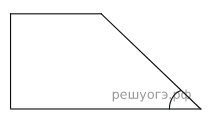
\includegraphics[align=t, width=\linewidth]{../../../../../exercises/lists/pics/leontevaM9L8-3}
         \end{minipage}
     	\item В трапеции \( ABCD \) \( AB  =  CD \), \( \angle BDA  =  49\degree \) и \( \angle BDC  =  13\degree \). Найдите угол \( ABD \). Ответ дайте в градусах.
     	\item В треугольнике \( ABC \) известно, что \( \angle BAC=82 \degree \), \( AD \)  --- биссектриса. Найдите угол \( BAD \). Ответ дайте в градусах.
     	\item К окружности с центром в точке \( О \) проведены касательная \( AB \) и секущая \( AO \). Найдите радиус окружности, если \( AB  =  45 \) , \( AO  =  75 \).
     	\item 
     	\begin{minipage}[t]{\bodywidth}
     		Окружность с центром в точке \( O \) описана около равнобедренного треугольника \( ABC \), в котором \( AB=BC \) и \( \angle ABC=123 \degree \). Найдите угол \( BOC \). Ответ дайте в градусах.
     	\end{minipage}
     	\hspace{0.02\linewidth}
     	\begin{minipage}[t]{\picwidth}
			% TODO: \usepackage{graphicx} required
			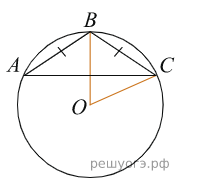
\includegraphics[align=t, width=\linewidth]{../../../../../exercises/lists/pics/leontevaM9L8-4}
     	\end{minipage}
     	\item
     	\begin{minipage}[t]{\bodywidth}
     		 Высота равнобедренной трапеции, проведённая из вершины \( C \), делит основание \( AD \) на отрезки длиной \( 17 \) и \( 19 \). Найдите длину основания \( BC \).
     	\end{minipage}
     	\hspace{0.02\linewidth}
     	\begin{minipage}[t]{\picwidth}
			% TODO: \usepackage{graphicx} required
			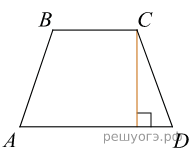
\includegraphics[align=t, width=\linewidth]{../../../../../exercises/lists/pics/leontevaM9L8-5}
     	\end{minipage}
     	\item Сторона треугольника равна \( 18 \), а высота, проведённая к этой стороне, равна \( 17 \). Найдите площадь этого треугольника.
     	\item 
     	\begin{minipage}[t]{\bodywidth}
     		На клетчатой бумаге с размером клетки \( 1\times 1 \) отмечены три точки: \( A \), \( B \) и \( С \). Найдите расстояние от точки \( A \) до середины отрезка \( BC \).
     	\end{minipage}
     	\hspace{0.02\linewidth}
     	\begin{minipage}[t]{\picwidth}
			% TODO: \usepackage{graphicx} required
			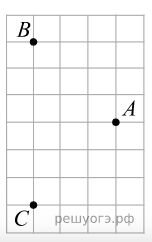
\includegraphics[align=t, width=\linewidth]{../../../../../exercises/lists/pics/leontevaM9L8-6}
     	\end{minipage}
     	\item Боковая сторона равнобедренного треугольника равна \( 5 \). Угол при вершине, противолежащий основанию, равен \( 120\degree \). Найдите диаметр окружности, описанной около этого треугольника.
     	\item Найдите площадь кругового сектора, если радиус круга равен \( 3 \), а угол сектора равен \( 120\degree \). В
     	ответе укажите площадь, деленную на \( \pi \).
     	\item В прямоугольнике диагональ равна \( 10 \), а угол между ней и одной из сторон равен \( 30\degree \). Найдите
     	площадь прямоугольника, делённую на \( \sqrt{3} \).
     	\item Какое из следующих утверждений верно?
     	\begin{tasks}(1)
     	\task  Отношение площадей подобных треугольников равно коэффициенту подобия.
     	\task  Диагонали прямоугольника точкой пересечения делятся пополам.
        \task Биссектриса треугольника делит пополам сторону, к которой она проведена.
     \end{tasks}
 	\item Укажите номера верных утверждений.
 	\begin{tasks}(1)
 		\task  Любые три прямые имеют не более одной общей точки.
 		\task  Если угол равен \( 120\degree \), то смежный с ним равен \( 120\degree \).
 		\task  Если расстояние от точки до прямой больше \( 3 \), то и длина любой наклонной, проведённой из данной точки к прямой, больше \( 3 \).
 	\end{tasks}
 	
 	
 	
	\end{listofex}
\end{class}
%END_FOLD